\part{Introduction}

Dans cette partie, nous décrirons les caractéristiques du projet et les technologies qui seront
employées pour le mettre en \oe uvre.

\section{Présentation du projet}

Le projet de stage proposé par l'entreprise 9h37 consiste à mettre en place un système de
sauvegarde et de sécurisation des données d'un réseau de partage. L'utilisateur devra être
apte à sauvegarder ses données simplement sur un service de partage sur le réseau LAN de
l'organisme. Ces données devront être sauvegardées et chiffrées sur un espace de stockage invisible
au reste du réseau. Enfin, elles devront être envoyées sur un hôte distant pour réaliser des backup
réguliers. Au sein de l'entreprise, une interface web permettant de gérer les données chiffrées
devra être mise en place.

Ce projet me permettra de développer des compétences en architecture réseau, en administration
de système \textit{UNIX}/\textit{Linux} et en développement web avec \textit{Python}/\textit{Django}.
L'apprentissage de méthode de chiffrement (\textit{GnuPG}) sera nécessaire à la réalisation du projet.
Les technologies de partage (\textit{Samba}) et de transfert (\textit{SSH}) seront approfondies.

L'enjeu de ce stage pour l'entreprise sera donc le développement d'une solution simple, efficace
et sécurisée pour répondre à la demande de leur client.

\paragraph{}
La demande à laquelle nous allons répondre peut se décomposer en quatre parties :

\begin{enumerate}
     \item Partage des données sur un réseau LAN interne à l'organisme.
     \item Sauvegarde et chiffrement des données sur un espace de stockage interne à l'organisme.
     \item Copie des données chiffrées chez un hôte distant (hébergeur, ...).
     \item Interface web de gestion des données chiffrées interne à l'organisme.
\end{enumerate}

\subsection{Partage des données}

La mise en place du partage de données permettra aux membres de l'organisme de mettre en commun
leur travail sur un espace de stockage partagé.

Cela implique la mise en place d'un serveur pour l'organisme.

Le partage doit être simple pour l'utilisateur et accessible à tout le réseau LAN.

\subsection{Sauvegarde et chiffrement des données}

Les données présentes sur le partage devront être sauvegardées et chiffrées.
Il faudra donc maintenir une liste des fichiers chiffrées présent sur l'espace de stockage
afin de ne pas chiffrer et sauvegarder plusieurs fois un même fichier.

L'espace de stockage n'est pas accessible sur le réseau LAN.

La sauvegarde et le chiffrement des données devra être périodique pour ne pas surcharger le
serveur et donc ne pas perturber le travail en cours dans l'organisme.

\subsection{Copie chez un hôte distant}

Le transfert devra être sécurisé. Il faudra maintenir une liste des fichiers présents sur l'hôte
distant afin de ne pas transférer plusieurs fois un fichier déjà à jour.

De même que pour la sauvegarde et le chiffrement, le transfert devra être périodique afin de ne
pas saturer la bande passante de l'organisme.

\subsection{Interface web}

L'interface web permettra de gérer les données chiffrées (les restaurer en cas de suppression
sur le partage, les supprimer, ...).

Celle ci se présentera sous la forme d'un navigateur de fichier classique, avec une arborescence,
une vue en icône/liste/... et une gestion simplifié des différentes actions sur les fichiers.

L'accès à cette application web devra être restreint aux membres de l'organisme ayant les autorisations
nécessaires pour la manipuler (la méthode d'authentification reste à déterminer).

\section{Schémas}

\subsection{Architecture réseau}

Pour l'architecture réseau, nous aurons donc :

\begin{description}
     \item[LAN] Un réseau local à l'organisme.
     \item[server] Un serveur interne à l'organisme.
     \item[partage] Un partage réseau sur le LAN de l'organisme.
     \item[stockage] Un espace de stockage interne.
     \item[remote] Un espace de stockage chez un hôte distant.
\end{description}

\paragraph{}
Voici un schéma simplifié des besoins du projet :

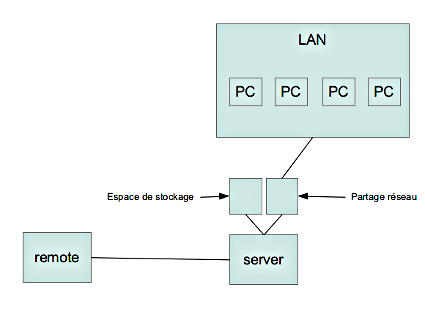
\includegraphics{img/schema01.png}

\subsection{Interface web}

L'interface web se présentera sous la forme d'un navigateur de fichier classique, elle devra donc
comporter les caractéristiques suivantes :

\begin{itemize}
     \item Arborescence de l'espace de stockage
     \item Vue en icône (ou liste) de l'espace de stockage
     \item Informations sur le fichier sélectionné
     \item Actions groupées (actions sur plusieurs fichiers)
\end{itemize}

Voici un exemple d'interface possible :

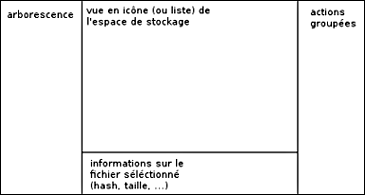
\includegraphics{img/schema02.png}

\section{Technologies utilisées}

Ici, on retrouvera la liste des technologies employées pour réaliser ce projet.

\subsection{Serveur}

\begin{description}
     \item[UNIX/Linux:] Système d'exploitation du serveur interne de l'organisme.
     \item[cron:] Utilitaire de programmation des tâches planifiées.
\end{description}

\subsection{Partage de données}

\begin{description}
     \item[Samba:] Service de partage réseau compatible \textit{UNIX} et \textit{Windows}.
\end{description}

\subsection{Sauvegarde et chiffrement}

\begin{description}
     \item[GnuPG:] Chiffrement asynchrone des données.
     \item[SQLite:] Base de données pour maintenir la liste des fichiers présents sur l'espace de stockage.
     \item[Python:] Le script sera intégré à \textit{Django}.
\end{description}

\subsection{Copie chez un hôte distant}

\begin{description}
     \item[scp:] Utilitaire de copie de données via \textit{SSH} (on utilisera des clés RSA, DSA ou EDSA pour l'identification).
     \item[SQLite:] Base de données pour maintenir la liste des fichiers présents sur l'hôte (on utilisera la base de données présente en locale).
\end{description}

\subsection{Interface web}

\begin{description}
     \item[Python:] L'interface web sera développé dans ce langage.
     \item[Django:] On utilisera ce framework pour le développement de l'application web.
     \item[Twitter Bootstrap:] Utilisé pour la construction de l'interface.
     \item[dajax \& dajaxice:] Pour la communication avec le serveur via AJAX.
\end{description}
